% Szglab4
% ===========================================================================
%
\chapter{Grafikus felület specifikációja}

\thispagestyle{fancy}

\section{A grafikus interfész}
\comment{A menürendszer, a kezelői felület grafikus képe. A grafikus felület megjelenését, a használt ikonokat, stb screenshot-szerű képekkel kell bemutatni. Az építészetben ez a homlokzati terv.}

\begin{figure}[h]
\begin{center}
%\includegraphics[width=17cm]{images/ch11/}
\caption{}
\label{fig:Grafikus}
\end{center}
\end{figure}

\section{A grafikus rendszer architektúrája}
%\comment{A felület működésének elve, a grafikus rendszer architektúrája (struktúra diagramok). A struktúra diagramokon a prototípus azon és csak azon osztályainak is szerepelnie kell, amelyekhez a grafikus felületet létrehozó osztályok kapcsolódnak.}

\subsection{A felület működési elve}
A grafikus felületet MVC architektúrának megfelelően próbáltuk megtervezni. Minden képernyőn megjelenő objektumnak van egy grafikus párja, ami megvalósítja a \textbf{Drawable} interfészt. A \textbf{View} osztály ilyen objektumokat tárol, és minden kirajzolásnál meghívja ezen objektumok draw metódusát. \\
A megjelenítés push alapú. Ha a modelben történt valami változás (amit hívhatunk egy eseménynek), akkor értesíti a \textbf{View}-t, hogy valami esemény történt, úgy hogy meghívja az eseménynek megfelelő metódust. Kirajzolásnál minden grafikus objektum, lekérdezi a \textbf{Game}-ben lévő párjától az adatait, majd ez alapján kirajzolja magát.\\
Az MVC megvalósítás alól kivételt képez a program indulása, amikor is egy egyszerű menü jelenik, amin el lehet indítani a játékot, ezt a \textbf{Menu} osztály végzi.\\
A \textbf{Controller} osztály a program elején, a \textbf{Game} és \textbf{View} objektumok létrehozása után feliratkozik a neki megfelelő eseményekre. Ez után már fogadja is az eseményeket.\\
Tervezés során ügyletünk arra is, hogy könnyen bővíthető, cserélhető legyen a rendszer. A \textbf{View} és \textbf{Graphic} osztályokból való származtatással új GUI-t lehet készíteni, anélkül, hogy meglévő kódban kelljen (sokat) változtatni.

\subsection{A felület osztály-struktúrája}
%\comment{Osztálydiagram. Minden új osztály, és azon régiek, akik az újakhoz közvetlenül kapcsolódnak.}

\begin{figure}[H]
\begin{center}
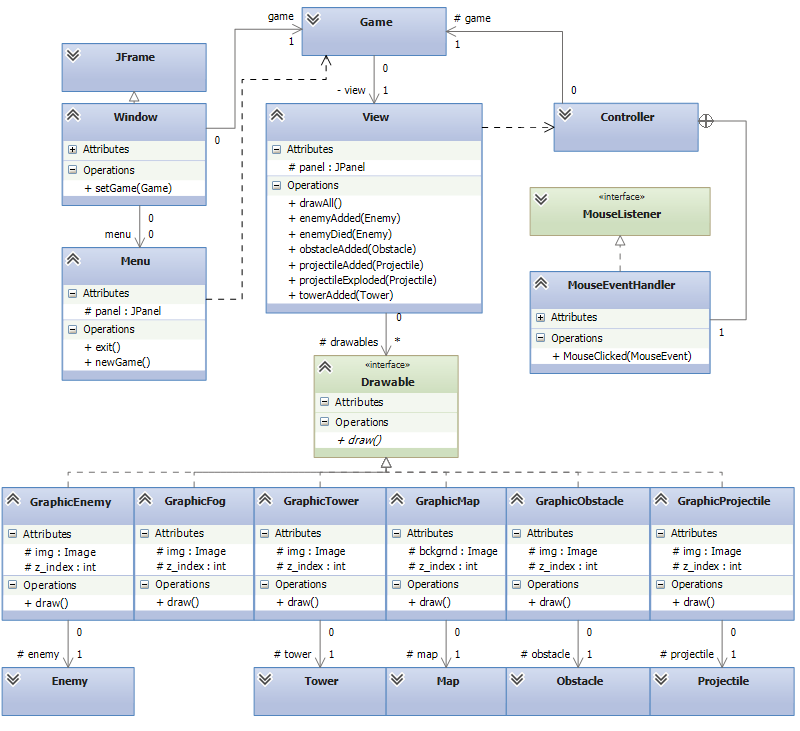
\includegraphics[width=18cm]{images/ch11/very_uml_class_tiny.png}
\caption{Grafikus felület osztálydigaramja}
\label{fig:Graphic_class_diag}
\end{center}
\end{figure}

\section{A grafikus objektumok felsorolása}
\comment{Az új osztályok felsorolása. Az régi osztályok közül azoknak a felsorolása, ahol változás volt. Ezek esetén csak a változásokat kell leírni.}

\subsection{Osztály1}
\begin{itemize}
\item Felelősség\newline
\comment{Mi az osztály felelőssége. Kb 1 bekezdés. Ha szükséges, akkor state-chart is.}
\item Ősosztályok\newline
\comment{Mely osztályokból származik (öröklési hierarchia)\newline
Legősebb osztály $\rightarrow$ Ősosztály2 $\rightarrow$ Ősosztály3...}
\item Interfészek\newline
\comment{Mely interfészeket valósítja meg.}
\item Attribútumok\newline
\comment{Milyen attribútumai vannak}
	\begin{itemize}
		\item attribútum1: attribútum jellemzése: mire való, láthatósága (UML jelöléssel), típusa
		\item attribútum2: attribútum jellemzése: mire való, láthatósága (UML jelöléssel), típusa
	\end{itemize}
\item Metódusok\newline
\comment{Milyen publikus, protected és privát  metódusokkal rendelkezik. Metódusonként precíz leírás, ha szükséges, activity diagram is  a metódusban megvalósítandó algoritmusról.}
	\begin{itemize}
		\item int foo(Osztály3 o1, Osztály4 o2): metódus leírása, láthatósága (UML jelöléssel)
		\item int bar(Osztály5 o1): metódus leírása, láthatósága (UML jelöléssel)
	\end{itemize}
\end{itemize}

\subsection{Osztály2}
\begin{itemize}
\item Felelősség\newline
\comment{Mi az osztály felelőssége. Kb 1 bekezdés. Ha szükséges, akkor state-chart is.}
\item Ősosztályok\newline
\comment{Mely osztályokból származik (öröklési hierarchia)\newline
Legősebb osztály $\rightarrow$ Ősosztály2 $\rightarrow$ Ősosztály3...}
\item Interfészek\newline
\comment{Mely interfészeket valósítja meg.}
\item Attribútumok\newline
\comment{Milyen attribútumai vannak}
	\begin{itemize}
		\item attribútum1: attribútum jellemzése: mire való, láthatósága (UML jelöléssel), típusa
		\item attribútum2: attribútum jellemzése: mire való, láthatósága (UML jelöléssel), típusa
	\end{itemize}
\item Metódusok\newline
\comment{Milyen publikus, protected és privát  metódusokkal rendelkezik. Metódusonként precíz leírás, ha szükséges, activity diagram is  a metódusban megvalósítandó algoritmusról.}
	\begin{itemize}
		\item int foo(Osztály3 o1, Osztály4 o2): metódus leírása, láthatósága (UML jelöléssel)
		\item int bar(Osztály5 o1): metódus leírása, láthatósága (UML jelöléssel)
	\end{itemize}
\end{itemize}

\section{Kapcsolat az alkalmazói rendszerrel}
\comment{Szekvencia-diagramokon ábrázolni kell a grafikus rendszer működését. Konzisztens kell legyen az előző alfejezetekkel. Minden metódus, ami ott szerepel, fel kell tűnjön valamelyik szekvenciában. Minden metódusnak, ami szekvenciában szerepel, szereplnie kell a valamelyik osztálydiagramon.}

